In this section, we choose four different supervised machine learning algorithms, and analyze their performance separately on the dataset. The best algorithm would be selected for implementation. \\

The algorithms chosen are as follows:

\begin{enumerate}
\item K-Nearest Neighbor Algorithm (KNN)
\item Support Vector Machine (SVM)
\item Gaussian Naive Bayes Classifier
\item Decision Tree Algorithm
\end{enumerate}

The results has been summarized in the following section. 

\subsection{Analysis}

The code used to build and compare the models discussed in this section has been uploaded in the project folder.

\subsubsection{K-Nearest Neighbor Algorithm (KNN)}

The k-nearest neighbors (KNN) algorithm is a supervised machine learning algorithm that can be used to solve both classification and regression problems. 

\\The algorithm was run on the dataset with varying values of k, and the best average accuracy gained was 0.83, with K-Fold Cross Validation, with the number of nearest neighbours as 3. \\

\begin{Figure}
  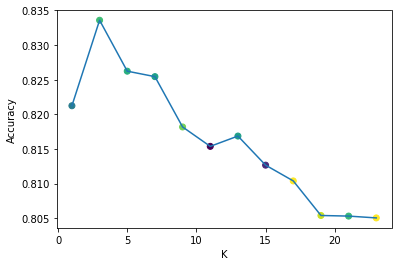
\includegraphics[width=\linewidth]{images/knn-accuracy.png}
  \captionof{figure}{Plot showing accuracy of KNN Algorithm with varying values of K}
  \label{fig:knnvaryingk}
\end{Figure}

\subsubsection{Support Vector Machine (SVM)}

Support vector machines (SVMs) are a set of supervised learning methods used for classification and regression problems. The Support Vector Machine algorithm gave an average accuracy of 0.77 with RBF Kernel. A lowest score of 0.65 was obtained with Sigmoid Kernel. \\

\begin{Figure}
  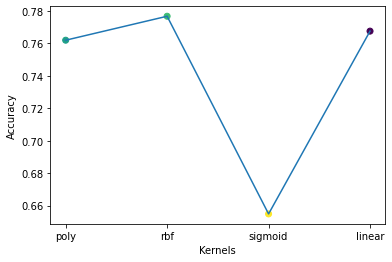
\includegraphics[width=\linewidth]{svm_accuracy}
  \captionof{figure}{Plot showing accuracy of SVM Algorithm with various kernels.}
  \label{fig:svmkernels}
\end{Figure}

\subsubsection{Gaussian Naive Bayes Classifier}

Gaussian Naive Bayes is a variant of Naive Bayes that follows Gaussian normal distribution and supports continuous data. \\

Gaussian Naive Bayes classifier yielded an average accuracy of 0.61. 

\subsubsection{Decision Tree Algorithm}

Decision Tree is a Supervised learning technique that can be used for both classification and Regression problem. It is a tree-structured classifier, where internal nodes represent the features of a dataset, branches represent the decision rules and each leaf node represents the outcome. \\

Decision Tree Algorithm yielded an average accuracy of 0.82. 

\subsection{Summary}

The results obtained from each algorithm has been summarized in the table below.

\begin{center}
\begin{minipage}[t]{.45\textwidth}
\begin{tabular}{@{}lllll@{}}
\toprule
\textbf{Algorithm}                  & Accuracy Obtained &  &  &  \\ \midrule
\textbf{KNN}                  & 0.83 &  &  &  \\ 
\textbf{SVM}                  & 0.77 &  &  &  \\
\textbf{Gaussian Naive Bayes} & 0.61 &  &  &  \\
\textbf{Decision Tree}                & 0.82 &  &  &  \\ \bottomrule
\end{tabular}
\end{minipage}
\end{center}

\begin{Figure*}
  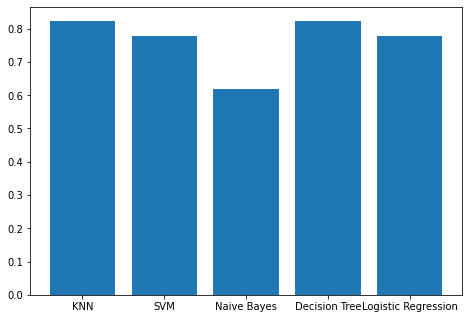
\includegraphics[width=\linewidth]{accuracy_comparison.png}
  \captionof{figure}{Comparison of various machine learning algorithms on the same dataset.}
  \label{fig:algocomparison}
\end{Figure*}


From the observations stated above, the KNN Algorithm appears as a best choice for this problem. We implemented KNN Algorithm, and the implementation has been discussed in the next section.

